% reviewers: Zam, Jared?

\documentclass{article}
\usepackage{graphicx}

\begin{document}

\title{Streaming approaches to error detection and trimming in the analysis of
short sequencing reads}
\author{TBD}
\maketitle

\section{Introduction}

K-mer spectral analysis is a powerful approach to error detection and
correction in shotgun sequencing data that uses k-mer abundances to
determine likely errors (cite Pevzner, Quake, khmer-counting paper).
Approaches derived from spectral analysis can be very accurate: Zhang
et al. (2014) show that spectral analysis is considerably more
effective at finding errors than quality-based approaches (cite).  However,
spectral analysis is also very compute intensive; most implementations
must count k-mers across entire sequencing data sets, which can be
memory- or I/O-intensive for large data sets.

Streaming algorithms can offer improved algorithmic and computational
efficiency in the analysis of large data sets (cite).  Streaming
algorithms typically examine the data only once, and scale in memory
usage sublinearly with respect to the input data.  Streaming
algorithms have not been applied to k-mer spectral analysis of reads,
although XXX (melsted).

Brown et al. (2012) introduced a streaming algorithm for normalizing
k-mer abundance spectra, termed ``digital normalization'' (abbreviated
as ``diginorm'').  This procedure estimates the k-mer coverage of each
read in an online algorithm, by calculating the median k-mer abundance
of the read given all previous reads; reads above a certain estimated
coverage are set aside and their k-mers are not tracked.  This
algorithm is both online and {\em streaming} because it only collects
k-mers in reads with a low estimated coverage; for the same reason, it
is sublinear in memory for high coverage data sets.  The net effect of
diginorm is to reduce the data set size that must be considered for
downstream processing, such as {\em de novo} assembly (cite trinity,
elijah, etc.)

Here we develop a streaming algorithm for k-mer spectral analysis,
based on digital normalization, that can detect and remove errors in
sequencing reads.  This algorithm operates in sublinear memory, and
examines the data at most twice.  The approach offers a general
framework for detecting and making use of graph saturation and could
potentially be used for error correction, variant calling, and
a streaming implementation of assembly.  Moreover, it can be applied to
data sets with variable coverage such as transcriptomes, metagenomes, and
amplified genomic DNA.

\section{Results}

\subsection{Coverage-normalized data can be used to locate
errors in high-coverage shotgun sequencing data}

To determine if digital normalization could be applied prior to k-mer
spectral error detection, we first generated a synthetic data set from
a simulated low-complexity genome (``simple genome''; see Methods for
generation and Table XXX for data set details).  We then applied
digital normalization to a median 20-mer coverage of 20 (k=20, C=20)
and used k-mer counts from the downsampled read set to detect errors
by looking for bases at the beginning or ends of low-abundance regions
in each read. We used a ``trusted k-mer'' cutoff of $C_0 = 3$ as our
abundance cutoff, below which we assumed k-mers were erroneous (see Methods).
% note, need to put in diginorm #s

Of the 531 reads in the simple genome with one or more errors,
predicted errors matched exactly for 317 of them (true positives), and
466 reads were correctly predicted to contain no errors (true
negatives). 90 reads were falsely predicted to have no errors (false
negatives). The errors in 124 reads were miscalled -- while the reads
each had one or more errors, the positions were not correctly called
-- and three reads were incorrectly predicted to contain errors,
leading to a total of 127 false positives.  Using the above
definitions, we calculated the prediction sensitivity to be 77.9\% and
the prediction specificity to be 71.4\%.

@@put in picture of k-mer abundance spectrum before and after?

@list in a table: matched exactly, etc. rundown.

% make ecoli-report.txt

We next applied digital normalization and k-mer spectral error
detection to an Illumina data set from E. coli MG1655 (cite Chitsaz).
We mapped 5m untrimmed reads to the known E. coli MG1655 genome with
bowtie1 (cite) and calculated mismatches between the reads and the
genome as errors in the reads.  This yielded 8.0m errors in 2.2m reads,
for an overall error rate of 1.60\%.  Using these errors as ground truth,
we found approximately 940,000 true positives, 2.8m true negatives,
895,000 false positives, and 356,000 false negatives.  This yielded
a sensitivity to errors of 72.4\% and a specificity of 51.1\%.

\subsection{Coverage-normalized data can be used to locate errors in variable
coverage shotgun sequencing data}

One of the drawbacks of spectral abundance analysis is that it cannot
be applied to metagenomic or transcriptomic data sets, which
frequently contain reads from both high-abundance and low-abundance
molecules.  This variability in coverage confounds naive spectral
analysis for two reasons: first, errors in very high abundance regions
can accumulate and increase over the threshold for trusted k-mers,
thus appearing to be correct; and second, correct reads from low
coverage regions yield k-mers below the trusted k-mer threshold and
appear to be incorrect.  In practice, therefore, error correction for
metagenomic and transcriptome data must use other approaches.

If we apply diginorm to variable coverage data, we address the problem
of accumulated errors from high-abundance regions by eliminating the
majority of the reads from these regions; this is a form of error
correction, detailed in the original diginorm paper (cite diginorm).
However, we can also address the issue of low-abundance regions by
ignoring reads that are as yet low coverage; here we can again use
the median k-mer abundance to estimate which reads are too
low-abundance to analyze (Figure XXX).

@graph with read abundance spectrum ,showing which reads we will
call errors in.

% make mcompare2
% make rcompare2

We generated two more synthetic data sets, ``simple metagenome'' and
``simple mRNAseq,'' which contain both high- and low-abundance species
(see Table XXX for data set details).  After generating synthetic
reads with a 1\% error rate and applying digital normalization to
k=20/C=20, we again applied spectral error detection
using the normalized counts, but with the modification that only reads
with a median k-mer abundance of 20 or greater were examined.  For the
simple metagenome data set, 2254 of 2347 reads (96.0\%) met the
coverage criterion.  Of the 2347 reads total, the errors in 658
erroneous reads were called perfectly (TP) and 1126 of the reads with
no errors were correctly called as error-free (TN).  297 reads were
incorrectly determined to be error free (FN; including the reads that
were too low coverage to be considered).  Of the remaining 266 reads,
261 were miscalled (errors existed but were not exactly called) and 5
were incorrectly called as erroneous when they were in fact correct.
We calculated the prediction sensitivity to be 68.9\% and the
prediction specificity to be 71.2\%.  For the simple mRNAseq data set,
524 of 568 reads (92.3\%) met the coverage criterion, with 153 true
positives, 255 true negatives, 87 false negatives (including the low
coverage reads not examined), and 73 false positives, for a prediction
sensitivity of 63.8\% and prediction specificity of 67.7\%.

@ real data / measurements

\subsection{A streaming algorithm can be used to detect errors based on read coverage}

Even with digital normalization, the spectral error detection approach
outlined above is a 2-pass offline algorithm for any given data set -
the first pass normalizes the read set and records the k-mer
abundances, while the second pass examines the reads.  A streaming
approach could avoid some or all of a second pass, leading to
greater efficiency.

Here we can make use of the redundancy of shotgun sequencing to avoid
examining much of the data twice. Shotgun
sequencing oversamples most regions -- for example, for a 100x
coverage genomic data set, we would expect 50\% or more of the genome
to be represented in more than 100 reads.  This is a consequence of
the Poisson-random sampling that underlies shotgun sequencing
(cite... Waterman?)  This oversampling provides an opportunity,
however; if we regard the read data set as a stream of incoming data,
some portions of the reference will more highly sampled earlier in the
stream than others.  For example, in mRNAseq, highly expressed
transcripts will on average be highly sampled much earlier than
low-expressed transcripts.

If highly sampled regions could be detected during iteration over the
read data set, we could apply the same approaches used above to do
error detection in a streaming fashion.  Digital normalization
provides such a method: by measuring coverage for each read against an
online De Bruijn graph, reads that reach a specified coverage
threshold can be examined for errors immediately.  Those reads that
had not yet reached high coverage could be set aside and re-examined
later.  This could result in significant runtime savings: for a
genomic data set with 100x coverage, no more than 20\% of the reads
would need to be examined twice.

The conceptual idea is presented in Figure XXX.

\begin{figure}[!ht]
 \centerline{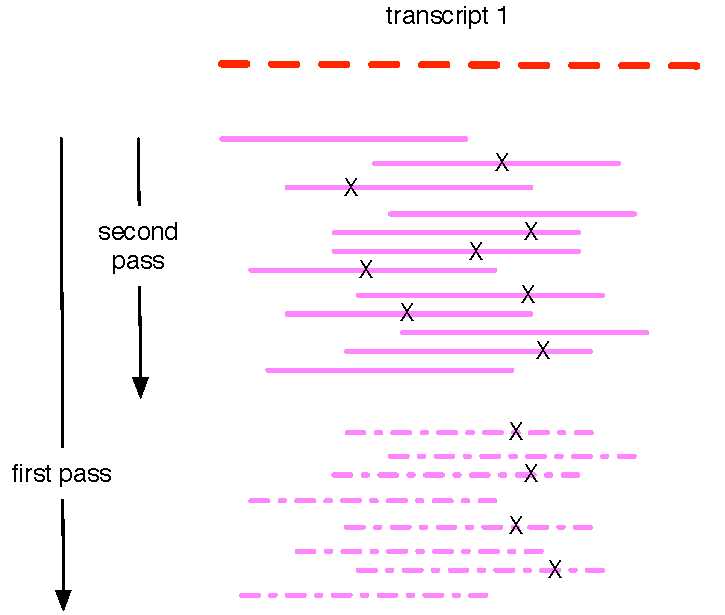
\includegraphics[width=4in]{./figures/graph-saturation}}
\caption{\bf Diagram of streaming error detection. In a first pass
over the read data, reads are loaded in until the graph locus to which
they belong is saturated.  From that point on, reads are examined for
errors and not loaded into the graph.  In a second pass, only the subset
of reads loaded into the graph are examined for errors.}
\label{fig:bar}
\end{figure}


In Figure XXX, we show diginorm-generated coverage saturation curves
for error-free simulated reads from synthetic and a real ({\em
  E. coli}) genome, as well as simulated reads with error from a
synthetic genome, and real reads from the {\em E. coli} genome.  In
all cases, we see that more than BLAH \% of reads reach an estimated
coverage of 20 no more than ZAH \% of the way through the data set.

% make compare4

%531 erroneous reads in simple-genome-stream-mismatches.pos
%531 erroneous reads in simple-genome-reads.mut.pos
%400 reads in common => all error positions AGREE
%128 DISAGREE
%total # of reads: 1000
%TP: 400
%TN: 466
%FP: 131
%FN: 3
%sensitivity: 0.992555831266
%specificity: 0.75329566855

When we apply this saturation-based approach to the simulated ``simple
genome'', we find 400 TP, 466 TN, 131 FP, and 3 FN, for a sensitivity
of 99.3\% and a specificity of 75.3\%.  (I don't know why this is better
than the full genome; massive decrease in FN? CTB.)

% make rcompare4
% 568
% 289 erroneous reads in mrna-stream-mismatches.pos
% 309 erroneous reads in mrna-reads.mut.pos
% 212 reads in common => all error positions AGREE
% 71 DISAGREE
% total # of reads: 568
% TP: 212
% TN: 253
% FP: 77
% FN: 26
% sensitivity: 0.890756302521
% specificity: 0.733564013841

% make mcompare4
% 2347
% 1116 erroneous reads in simple-metagenome-stream-mismatches.pos
% 1216 erroneous reads in simple-metagenome-reads.mut.pos
% 876 reads in common => all error positions AGREE
% 235 DISAGREE
% total # of reads: 2347
% TP: 876
% TN: 1126
% FP: 240
% FN: 105
% sensitivity: 0.892966360856
% specificity: 0.784946236559

Likewise, when we apply the approach to the simulated ``simple
metagenome'' and ``simple mRNAseq'' data sets, we achieve
sensitivity/specificity to the precise locations of errors in reads of
89.3\% and 78.5\% on the metagenome and 89.1\%/73.4\% on the mRNASeq
(see Table YYY for details).

@ discuss streaming error detection results.

\subsection{A streaming algorithm for error trimming}

We can now implement a streaming algorithm for error {\em trimming} of
any shotgun data.  This follows directly from streaming error
detection: instead of identifying the locations of {\em all} errors,
we truncate the read at the {\em first} (5') low abundance k-mer.
(While it is possible to split reads around errors rather than
truncating them, this introduces complications in downstream read
processing.)

On the ``simple genome'' with counts from the digitally normalized reads,
this trimming approach eliminates 149 reads entirely due to a starting
low-abundance k-mer, and truncated another 392 reads.  Of the 100,000
bp in the simulated reads, 31,910 (31.9\%) were removed by the
trimming process.  In exchange, trimming eliminated all of the errors,
bringing the overall error rate from 0.63\% to 0.00\%.

For the simple metagenome we used the variable abundance approach
described above and only trimmed reads with estimated coverage of 20
or higher.  Here, of 2347 reads containing 234,700 bp, 314 reads
(13.4\%) were removed and 851 reads (36.3\%) were trimmed, discarding
a total of 74,321 bases (31.7\%).  Of 1451 errors total, all but 61
were eliminated, bringing the overall error rate from 0.62\% to
0.04\%.  The simple mRNAseq data set showed similar improvement: 83 of
568 reads were removed, and 208 were trimmed, removing 19,507 of
56,800 bases (34.34\%).  The initial error rate was 0.65\% and the
final error rate was 0.07\%.

% ecoli-report-untrim.txt ('make ecoli-report-untrim.txt')
%posfile ecoli-reads.sam.pos: 2176576 mutated reads of 5000000; 7952048 mutations total
%500000000 bp total
%overall error rate: 1.590410%

% ecoli-report-trim.txt ('make ecoli-report-trim.txt')
%posfile ecoli-abundtrim.sam.pos: 171582 mutated reads of 4878226; 198192 mutations total
%435223632 bp total
%overall error rate: 0.045538%

% output of make ecoli_ref-5m.fastq.gz.abundtrim
%read 5000000 reads, 500000000 bp
%wrote 4878226 reads, 435223632 bp
%removed 121774 reads and trimmed 2046584 reads
%trimmed or removed 12.96% of bases (64776368 total)
%output in *.abundtrim

Applying the streaming error trimming to the E. coli MG1655 data set
used in section XXX, we trimmed 2.0m reads and removed nearly 122,000
reads entirely.  Of 7.6m errors, all but 198,000 were removed,
bringing the error rate from 1.60\% to 0.5\%.  Trimming discarded 64
Mbp of the original 500 Mbp (13.0\%).

@ mrna
@ real metagenome

\subsection{Illumina error rates and error profiles can be determined from a
small sample of sequencing data}

With Illumina sequencing, average and per-position error rates may
vary between sequencing runs, but are typically systematic within a
run (cite?).  Per-position error rates are caused by fluidics etc.

We can use the approaches described above to calculate systematic
error profiles for shotgun sequencing data across entire data sets,
but the variable abundance approach developed above can also be
applied to {\em subsets} of Illumina data.  The essential idea is to
consume reads until sufficient data has been collected to calculate
error rates, and then to calculate those error rates for the new reads
based on the k-mer abundances from the old reads.  This can aso be
done in one pass for data sets with sufficiently high coverage data:
as shown above (Figure XXX), more than half of the reads will have
sufficient coverage to call errors by the time 10\% of the data set
has been consumed.

We first simulated a set of reads from the simple genome with errors
only at even positions (0, 2, 4, etc.), and called errors in these
reads using the single-pass algorithm described above (see Methods for
implementation details).  We also separately called errors by mapping
with bowtie and examining mismatches.  The results are shown in Figure
YYY; the difference in predicted vs actual mismatch profiles has an
average of 0.04\%, with a variance of 0.0002\% across positions.  The
predicted per-base error rate is 0.57\%, while the true error rate is
0.65\%; this underestimate may be due to ignoring reads with multiple
errors in them that present as too low-coverage to assess.

@@show figure with shaded color indicating difference

We next applied to ecoli data.@@

@@error rates? apply regression?

\section{Discussion}

\subsection{Digital normalization enables k-mer spectral error detection in fariable abundance shotgun data}

Reference-free error detection and correction in shotgun data from
metagenomic, transcriptomic, and amplified samples typically requires
specialized approaches (cite, discuss).  Here we demonstrate
that after digital normalization, k-mer abundance spectral approaches
can be applied to reads estimated to have high coverage.  This should
generalize to any error detection, trimming, and counting approaches
that rely on k-mer abundance.

One significant disadvantage of the variable abundance approach is
that low-coverage reads cannot be trimmed because we do not know
whether they are from low-abundance molecules or are highly erroneous.
This must be taken into account for downstream analysis; for example,
while assemblers must already ignore or correct these erroneous reads,
quantitation approaches using e.g. mapping should be not be applied
to the trimmed data.

(@This is where applying Quake would be a useful demonstration.)

% Will this apply to all error correctors?
% -V means that highly erroneous reads are kept, but htye're all low coverage.

\subsection{Read coverage estimates enable streaming few-pass approaches to error detection and trimming}

K-mer spectral error detection and trimming approaches require two
complete passes through the data - one for calculating k-mer
abundances, and one for trimming reads.  Here we develop an approach
to streaming error detection and trimming that relies on uneven
coverage saturation as the read data set is traversed.  Again, this
approach should be general.

%Will this apply to all error correctors?

%The kind of trimming we implement is only useful for lower memory
%assembly, etc. Should not be used prior to quantification assembly as
%it will bias against high cov.

\subsection{Empirical error profiles can be calculated on subsets of Illumina shotgun data}

Useful for cores etc: quick evaluation of sequencing quality, regardless
of origin.

\subsection{Concluding thoughts}

Primary practical - The kind of trimming we implement is only useful
for low memory assembly of variable coverage data sets, but we have
plenty.

Time- and memory-efficient error profile calculation is practically useful
for large sequencing cores.

Dealing with variants is outside the scope of this work, but 50/50
variants should not be trimmed.  What about repeats?

Streaming methods for error correction and variant calling, more generally.

Theory needed for thresholding, but, in theory, thresholds should be
static.  (We can demonstrate that there is little variation.?

\end{document}
